\section{Architettura}\label{architettura}
\subsection{Scopo del Capitolo}
Lo scopo del capitolo è quello di fornire le informazioni necessarie allo sviluppatore per potersi interfacciare con il prodotto, in modo tale da rendere più agevole l'ampliamento e la modifica.

\subsection{Pannello}\label{archPannello}
Per rendere lo sviluppo più semplice, e garantire la manutenibilità del codice il team ha optato per un approccio modulare. In questo modo, avendo moduli separati con compiti distinti, sarà più semplice modificarne o estenderne il comportamento senza dover necessariamente modificare la base comune.\\
In particolare i moduli separati sono:
\begin{itemize}
	\item \textbf{GBCtrl}: è il modulo principale che utilizza gli altri e svolge le operazioni fondamentali;
	\item \textbf{TemporalPolicyCtrl}: è il modulo che si occupa di gestire ed impostare le politiche temporali all'interno del pannello;
	\item \textbf{ThresholdsCtrl}: è il modulo che si occupa di gestire ed impostare le soglie per il monitoraggio;
	\item ...
\end{itemize}

\subsubsection{UML}
\begin{figure}[H]
\begin{center}
	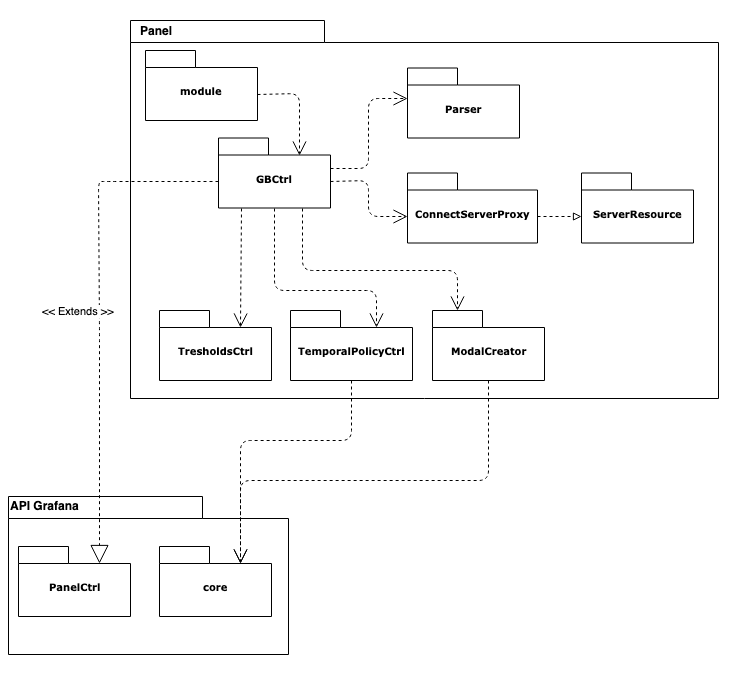
\includegraphics[scale=0.6]{./images/panelPackage.png} 
\end{center}
\caption{Diagramma dei Package del Pannello}
\end{figure}


\subsection{Server}\label{archServer}
\subsubsection{UML}
\begin{figure}[H]
	\begin{center}
		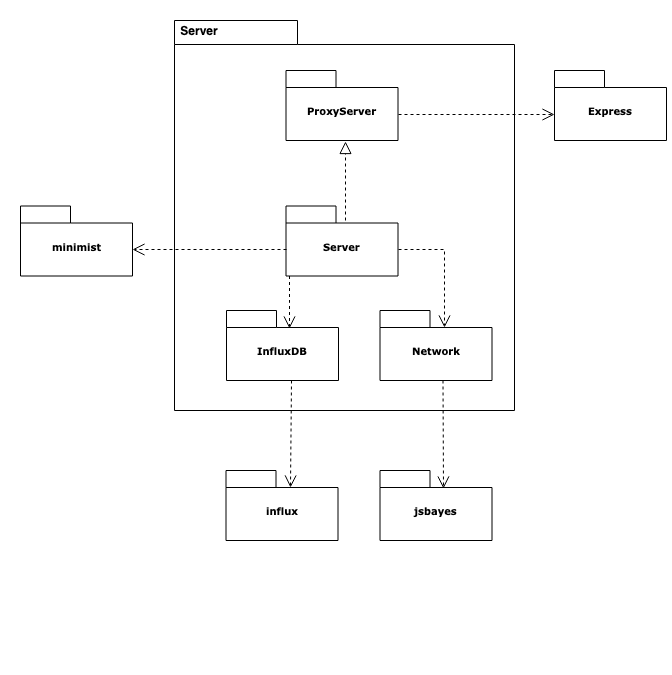
\includegraphics[scale=0.6]{./images/serverPackage.png} 
	\end{center}
	\caption{Diagramma dei Package del Pannello}
\end{figure}

